\documentclass{beamer}
\usetheme{Boadilla}
\usepackage{essay-def}
\usepackage{bm}
\usepackage{amsfonts}
\usepackage{amssymb}
\usepackage{amsmath}
\usepackage{amsthm}
\usepackage{comment}
\usepackage{geometry}
\geometry{left=1cm,right=1cm}
    \title[Distribution Mismatch]{On distribution mismatch in Data-driven Scientific Computing}
\author[J. Zhao]{Jiaxi Zhao}
\date{16th August, 2022}
\begin{document}
\par \setlength{\parindent}{2em}

\begin{frame}
\titlepage

\end{frame}


\begin{comment}
\begin{frame}{What is turbulence?}
    \begin{figure}[H]
          \centering
          \centerline{\includegraphics[width=\linewidth]{turbulence.png}}
        \end{figure}
\end{frame}


\begin{frame}{What is turbulence?}
	Turbulence appears in nearly everywhere of our life:
	\begin{itemize}
		\item 1. design of the car and airplane
		\item 2. swimming
		\item 3. cooking
	\end{itemize}
	Some times one wishes to eliminate the turbulence, i.e. design of the airfoil (wings of the plane); some times one would like to promote it, i.e. mixing of the solution and transfer of the heat.
\end{frame}

\begin{frame}{How do we model and study turbulence?}
	In the fluid mechanics society, research on turbulence had a long history. With the contribution from Newton, Onsager, Prandtl, and many more outstanding researchers, nowadays people have well-developed model and tools to study turbulence. Here are several approaches:
	\begin{itemize}
		\item 1. Navier-Stokes (NS) equation (Euler equation).
		\item 2. Boltzmann equation.
		\item 3. Theory of boundary layer.
	\end{itemize}
\end{frame}


\begin{frame}{The need of turbulence modeling}
	Recall the incompressible NS equation is written as
	\bequn
		\begin{aligned}
			\nabla \cdot \mfU & = 0,		\\
			\p_t \mfU + (\mfU \cdot \nabla)\mfU & = \nu \Delta \mfU - \frac{1}{\rho}\nabla p.		\\
		\end{aligned}
	\eequn
	The Reynolds number is defined as $\frac{U_0 L_0}{\nu}$. When the Reynolds number is big, the flow behaves chaotic with multi-scale. Below is a typical snapshot of the velocity field in a high-Reynolds fluid:
	\begin{figure}[H]
          \centering
          \centerline{\includegraphics[width=0.75\linewidth]{snapshot.png}}
        \end{figure}
\end{frame}


\begin{frame}{RANS}
	In this talk we will focus on one kind of turbulence modeling related to the Reynolds average Navier-Stokes (RANS) equation. Denote by $\la \mfU \ra$  the time average of $\mfU$ and $\mfu = \mfU - \la \mfU \ra$:
	\bequ
	\p_t \la \mfU \ra + (\la \mfU \ra \cdot \nabla)\la \mfU \ra + \frac{\p \la \mfu u_j \ra}{\p x_j} = -\frac{1}{\rho}\nabla p + \nu \Delta \la \mfU \ra,
\eequ
An extra term comes in, i.e. $\la \mfu u_j \ra$ Reynolds stress. The equation is no longer close!!
\end{frame}


\begin{frame}{RANS}
	One of the most famous model for the Reynolds stress is the eddy-viscosity hypothesis:
	\bequ
	-\la u_iu_j \ra = \nu_t \lp \frac{\p \la U_i \ra}{\p x_j} + \frac{\p \la U_j \ra}{\p x_i} \rp - \frac{2}{3}\delta_{ij}k,
	\eequ
	where $k = u_iu_i$ the turbulent kinetic energy. Based on this assumption, Reynolds stress contributes to viscosity term by an eddy-viscosity (turbulent viscosity). And closing the equation transfers to calculate the eddy-viscosity $\nu_T$.
	\begin{itemize}
		\item 1. One equation model
		\item 2. Two equation model: k-$\varepsilon$, k-$\omega$.
	\end{itemize}
\end{frame}


\begin{frame}{Data-driven method}
	An effective approximation related the Reynolds stresses to a basis of tensors $T^{(1)}, T^{(2)}, \cdots, T^{(10)}$. This tensor are designed to guarantee several invariance of the fluid statistics.
	\bequ
	\mathbf{b} = \sum_{n=1}^{10} g^{(n)}(\lambda_1, \lambda_2, \cdots, \lambda_5) T^{(n)}.
\eequ
\end{frame}


\begin{frame}{Data-driven method}
	\begin{figure}[h]
	\centering
  	\includegraphics[width=0.8\linewidth]{590-590.png}
  	\caption{Interpolation in Re590}
  	\label{590-590}
\end{figure}
\end{frame}


\begin{frame}{Inner-outer loop: linear case}
	The key feature of linear-outer loop is that error in the computation of inner loop can be propagated by outer loop, and gradually affect the trajectory of the dynamics, which is what we are primarily concerned with. We first restrict our attention to the case where inner loop is also linear, i.e.
	\begin{align}\label{linear-sys}
	\mfX_{k+1} & = A\mfX_{k} + B\mfZ_k,\quad \mfX_k \in \mbR^n, \mfZ_k \in \mbR^m,		\nonumber \\
	\mfZ_k & = C\mfX_k.
\end{align}
\end{frame}


\begin{frame}{Inner-outer loop: linear case}
	\begin{Prop}[DRO of linear regression]\label{linreg-DRO}
	Consider the DRO formulation of linear regression in special case where $\Cov(\mfX) = \Sigma, \mu \in \mcN(\mu_0, \varepsilon) = \lbb \Sigma_0 + \Delta \Sigma | \norml \Delta \Sigma \normr_2 \leq \delta \rbb$:
	\bequ\label{DRO}
	\Theta = \arg\min_{\theta} \sup_{\mu \in \mcN(\mu_0, \varepsilon)} \mbE_{X \sim \mu} \norml \mfY - \theta \mfX \normr^2,
\eequ
	It is equivalent to the following regularized problem
	\bequ\label{regularize}
	\Theta = \arg\min_{\theta} \mbE_{\mfX \sim \mu} \norml (C - \theta) \mfX \normr^2 + \delta\norml S \normr_*,
\eequ
where $S = (C^T - \theta^T)(C - \theta).$
\end{Prop}
\end{frame}


\begin{frame}{Inner-outer loop: linear case}
	The influence of inner loop to the whole trajectory statistics can be indicated in the structure of covariance.
	\begin{Prop}[Distribution shift of the linear dynamics]\label{dyn-DRO}
	Consider the special case where $E$ commutes with $E^T$. Then the distribution shift associated with model shift $E \rightarrow E+\Delta E$ is given by
	\bequ\label{dyn-regularize}
	\begin{aligned}
	\sup_{\Delta E}& \sum_{k = 0}^N 2(N-k)f_{k, l}		\\
	f_{k, l} = & \Tr(E^T (E^{l})^T (EE^T)^{k-l-1} S E^l \Delta E ),
	\end{aligned}
\eequ
where $S = (C^T - \theta^T)(C - \theta).$ If further either $\Delta E$ or $S$ is assumed to commute with $E, E^T$, this reduces to 
\bequ
\Tr(\sum_{k = 0}^N 2k(N-k)E^T (EE^T)^{k-1} S\Delta E)
\eequ
\end{Prop}
\end{frame}


\begin{frame}{Inner-outer loop: non-linear case}
	For nonlinear case, the shift of covariance structure is no longer in closed-form, but we can still use some methods to obtain some informations in the covariance shift.
	\begin{itemize}
		\item 1. linearization
		\item 2. adjoint equation
		\item 3. integrable models
	\end{itemize}
\end{frame}


\begin{frame}{Inner-outer loop: non-linear case}
\begin{Ex}[Generalized linear model]
First example is a generalized linear model where the basis $\phi_i$ is taken to be known.
\bequ
\begin{aligned}
	& \min \mcF		\\
	& s.t. \  \dot{\mfX}_t = \sum_{i=1}^n \alpha_i \phi_i(\mfX_t).
\end{aligned}
\eequ
Then use the method of adjoint equation, we can calculate the derivative of $\mcF$ w.r.t. the parameter $\alpha$:
\bequn
	\nabla_{\alpha} \mcF = \frac{1}{\tau}\int_0^{\tau}(\mfX_t^T\nabla\phi_i(\mfX_t)\mathbf{\lambda_t} - \phi_i(\mfX_t)^T\mathbf{\lambda_t})dt.
\eequn
\end{Ex}
\end{frame}


\begin{frame}{Inner-outer loop: non-linear case}
	\begin{Ex}[Gibbs measure]
Another example is the Gibbs measure, which is important in sampling problem. Suppose the ground-truth distribution is given by the following Gibbs measure $\frac{1}{\mcZ_0^2}e^{-V_0(\mfX)}$, then a shift of the potential $V_{\varepsilon}(\mfX) = V_0(\mfX) + \varepsilon \bsyb \eta(\mfX)$ will cause the following covariance shift.
\bequn
	\begin{aligned}
		\Cov_{\varepsilon}(\mfX) = & \ \frac{\int_{\mfX} \mfX\mfX^T e^{-V_{\varepsilon}(\mfX)}d\mfX}{\mathcal{Z}_{\varepsilon}}		\\
		= & \ \Cov_0(\mfX) + \frac{\int_{\mcX} e^{-V_0(\mfX)}\bsyb \eta(\mfX)d\mfX\int_{\mcX} \mfX\mfX^Te^{-V_0(\mfX)}d\mfX}{\mcZ_0^2} -  \\
		& \ - \frac{\int_{\mcX}e^{-V_0(\mfX)}d\mfX\int_{\mcX} \mfX\mfX^Te^{-V_0(\mfX)}\bsyb \eta(\mfX)d\mfX}{\mcZ_0^2}
	\end{aligned}
\eequn
\end{Ex}
\end{frame}


\begin{frame}{Performance of different estimators}
	Estimation in this inner-outer loop structure is completely different from that of traditional least square estimation and system identification. For linear system identification, satisfying statistical results have been establish for both stable and unstable system while nonlinear system is still beyond our knowledge.
\end{frame}


\begin{frame}{Performance of different estimators}
	We considering the following estimators in our experiments for linear inner loop:
	\begin{itemize}
		\item 1. Ordinary least square
		\item 2. Ridge least square
		\item 3. Lasso least square
		\item 4. One-step ordinary least square
		\bequn
			\min \norml \mfZ_k - \theta \mfX_k \normr^2 + \lambda\norml \mfX_{k+1}(\theta) - \theta \mfX_{k+1} \normr^2.
		\eequn
	\end{itemize}
\end{frame}
\end{comment}


\begin{frame}{Data-driven scientific computing}
	Data-driven method is becoming a prevalent surrogate model in mathematical modeling and scientific computing, due to its power on approximation the data in complicated and high dimensional setting.
	\begin{figure}[H]
          \centering
          \centerline{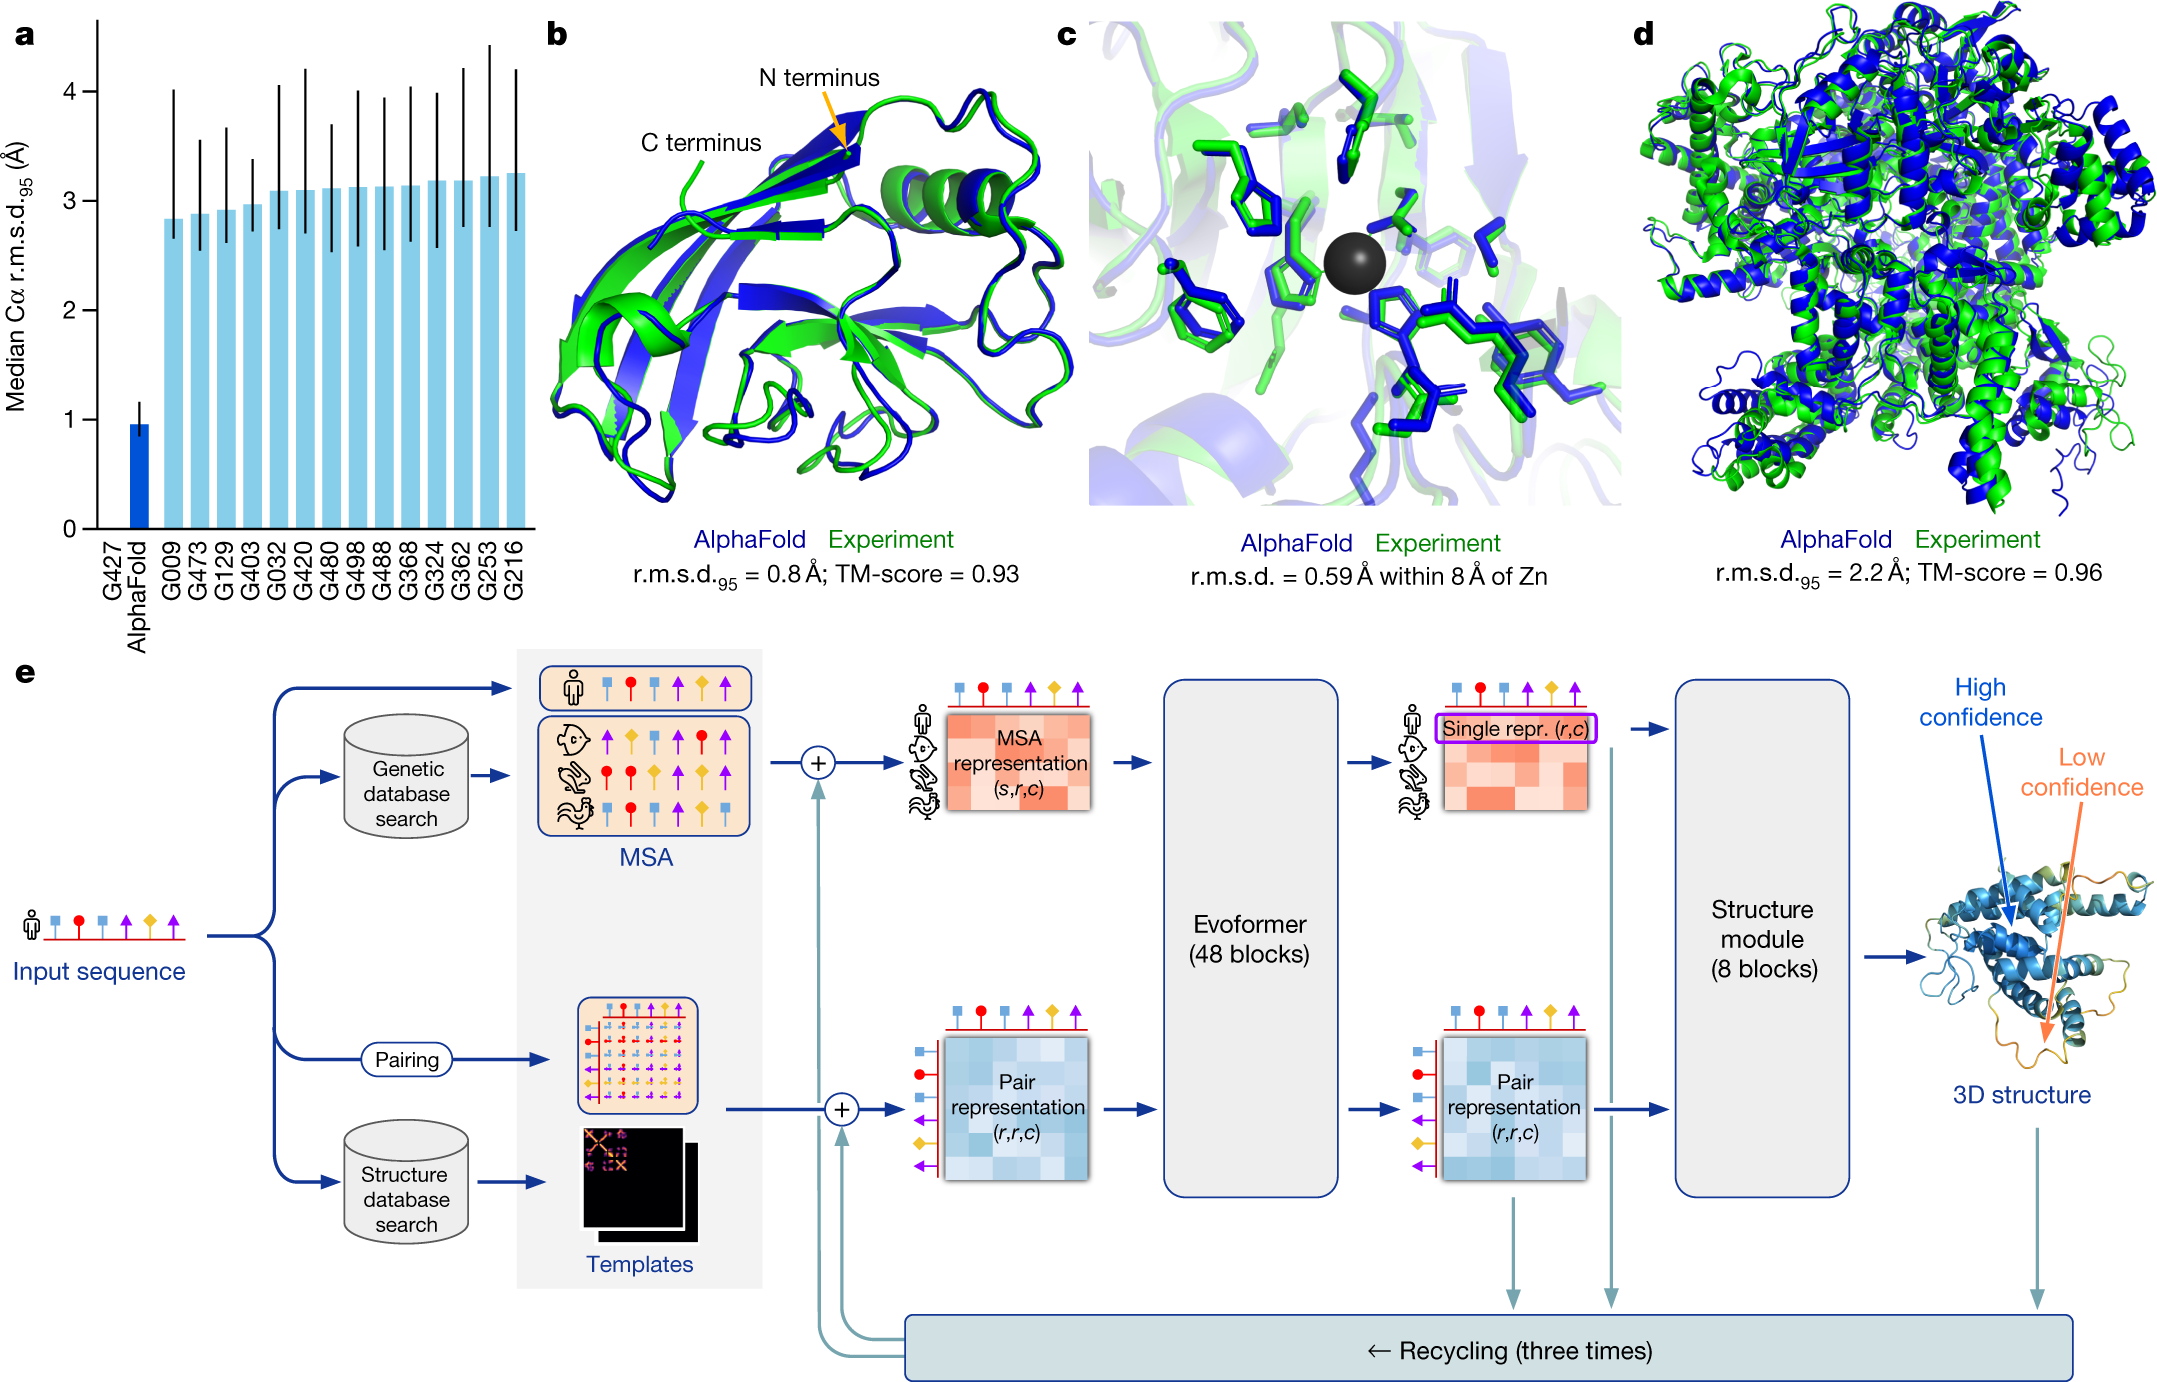
\includegraphics[width=0.7\linewidth]{fig/alphafold.png}}
        \end{figure}
\end{frame}


\begin{frame}{Data-driven scientific computing: Three Categories}
	\begin{itemize}
		\item 1. \textbf{100\% data-driven}: Physics-informed neural networks (PINN), Fourier neural operator, DeepONet.
		\item 2. \textbf{50 \% Numerical + 50 \% data-driven}: Machine learning turbulence modeling, DeepPotential, Quasipotential. 
		\item 3. \textbf{Discovering physics law from data}: Symbolic regression for conservation law, Principle component analysis for phase transition, cluster algorithm for space-time classification.
	\end{itemize}
\end{frame}


\begin{frame}{PINN's formulation}
	Numerical PDE $\Longrightarrow$ \textcolor{red}{\textbf{Regression problem}}\footnotemark with regularization:
	\bequn
		\begin{aligned}
		\Delta u(x) & = f(x) \quad x \in \Omega, \quad u(x) = g(x) \quad x \in \p \Omega.		\\
		\arg\min_u & \sum_{i=1}^{N_i} |\Delta u(X_i) - f(X_i) |^2 + \sum_{i=1}^{N} | u(Y_i) - g(Y_i) |^2, \\
		& X_i \in \Omega, Y_i \in \Omega \cup \p \Omega.
		\end{aligned}
	\eequn
	\par
	Satisfying performance for inverse problem!
\footnotetext{Raissi, Maziar, Paris Perdikaris, and George E. Karniadakis. "Physics-informed neural networks: A deep learning framework for solving forward and inverse problems involving nonlinear partial differential equations." Journal of Computational physics 378 (2019): 686-707.
}
\end{frame}


\begin{frame}{PINN for Boussinesq equation}
	\bequn
		\begin{aligned}
			\p_t u + u \cdot \nabla u + \nabla p = (0, -\theta), \quad 
			\p_t \theta + u \cdot \nabla \theta = 0.
		\end{aligned}
	\eequn\begin{figure}[H]
          \centering
          \centerline{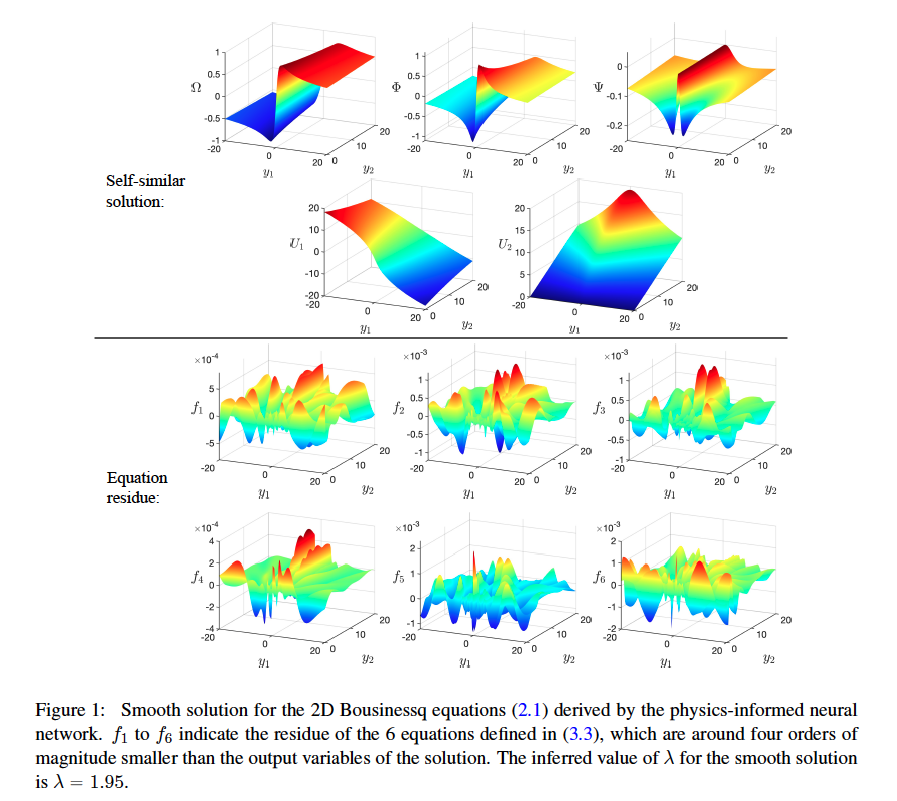
\includegraphics[width=0.5\linewidth]{fig/PINN-NS.png}}
        \end{figure}
\footnotetext{Wang, Yongji, et al. "Self-similar blow-up profile for the Boussinesq equations via a physics-informed neural network." arXiv preprint arXiv:2201.06780 (2022).
}
\end{frame}


\begin{frame}{Data-driven for Reynolds stresses modeling}
	$\la \mfU \ra =$ time average of $\mfU$, $\mfu = \mfU - \la \mfU \ra$, Reynolds-averaged Navier-Stokes (RANS) equation reads
	\bequ
		\begin{aligned}
	\p_t \la \mfU \ra + (\la \mfU \ra \cdot \nabla)\la \mfU \ra + \frac{\p \la \mfu u_j \ra}{\p x_j} &= -\frac{1}{\rho}\nabla p + \nu \Delta \la \mfU \ra,		\\
	\nabla \cdot \la \mfU \ra &= 0.
	\end{aligned}
\eequ
Extra term: $\la \mfu u_j \ra$ (Reynolds stress). \textcolor{red}{\textbf{The equation is not closed}}!!
\par
Ling et al.\footnotemark proposed a data-driven surrogate model to estimate the Reynolds stresses.
\footnotetext{Ling, Julia, Andrew Kurzawski, and Jeremy Templeton. "Reynolds averaged turbulence modelling using deep neural networks with embedded invariance." Journal of Fluid Mechanics 807 (2016): 155-166.
}
\end{frame}


\begin{frame}{Improve the prediction of flow separation}
	\begin{figure}[H]
          \centering
          \centerline{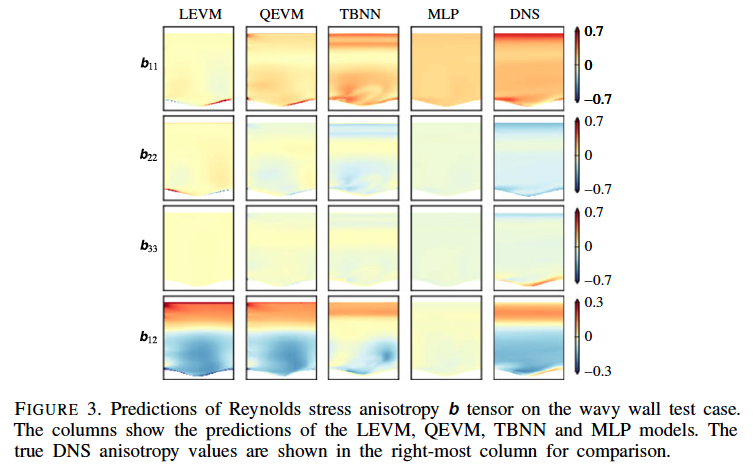
\includegraphics[width=\linewidth]{fig/tbnn.png}}
        \end{figure}
\end{frame}


\begin{frame}{Data-driven scientific computing: Our Focus}
	\begin{itemize}
		\item 1. \textbf{100\% data-driven}: Physics-informed neural networks (PINN), Fourier neural operator, DeepONet.
		\item 2. \textcolor{red}{\textbf{50 \% Numerical + 50 \% data-driven}: Machine learning turbulence modeling, DeepPotential, Quasipotential.} 
		\item 3. \textbf{Discovering physics law from data}: Symbolic regression for conservation law, Principle component analysis for phase transition.
	\end{itemize}
\end{frame}


\begin{frame}{Framework for the second approach}
	Simulating the dynamics:
	\bequn
		\begin{aligned}
			\p_t \mfx & = \mcL(\mfx, \mfu, t), \quad \mfx \in \mcX, \mfu \in \mcU, \mcL: \mcX \times \mcU \times \mbR_+ \rightarrow T\mcX,			\\
			\mfu & = \phi(\mfx, t), \quad \phi: \mcX \times \mbR_+ \rightarrow \mfu.
		\end{aligned}
	\eequn
	\begin{itemize}
		\item 1. $\mcL$ is known, possibly non-linear.
		\item 2. $\phi$ is un-known.
		\item 3. A set of data pairs $\lbb (\mfx_1, \mfu_1, t_1), (\mfx_2, \mfu_2, t_2), \cdots, (\mfx_N, \mfu_N, t_N )\rbb. $
		\item 4. Benchmark algorithm solves the ordinary least square:
		\bequn
			\arg\min_{\theta} \mbE \norml \mfu - \phi_{\theta}(\mfx, t) \normr^2.
		\eequn
	\end{itemize}

\end{frame}


\begin{frame}{Inner-outer loop: Linear outer loop}
In many scientific computing examples, further simplification:
\begin{align*}\label{linear-sys}
	\mfx_{k+1} & = A\mfx_{k} + B\mfu_k,\quad \mfx_k \in \mbR^n, \mfu_k \in \mbR^m,		\nonumber \\
	\mfu_k & = f(\mfx_k).
\end{align*}
\par
The outer loop is known to us and usually has some good numerical properties, i.e. linear, stable, etc, while the inner loop can be complicated.
\end{frame}


\begin{frame}{Inner-outer loop: examples}
\begin{Ex}[RANS]
\bequn
	\begin{aligned}
&\left\{\begin{aligned}
	\p_t \la \mfU \ra + (\la \mfU \ra \cdot \nabla)\la \mfU \ra + \nabla \cdot \tau &= -\frac{1}{\rho}\nabla p + \nu \Delta \la \mfU \ra,		\\
	\nabla \cdot \la \mfU \ra &= 0.
\end{aligned}\right.		\\
&\tau = R(\la \mfU \ra).
\end{aligned}
\eequn
\end{Ex}
\begin{Ex}[Quasi-potential]
\begin{align}\label{qp}
	\mfx_{k+1} & = \mfx_{k} - \Delta t\mfu_k,		\nonumber \\
	\mfu_k & = \nabla V_{\theta}(\mfx_k) + g_{\theta}(\mfx_k).
\end{align}
\end{Ex}

\end{frame}


\begin{frame}{Imitation learning}
	This structure also appears in \textcolor{red}{\textbf{reinforcement learning}} problems, or more specifically: \textcolor{red}{\textbf{imitation learning}}.
	\begin{Def}
		For a system with transition model $p(x_t | x_{t-1}, u_{t-1})$ with states $x \in \mcX$ and controls $u \in \mcU$, the imitation learning problem is to
leverage a set of demonstrations $\Xi = \lbb (x_0, u_0, t_0), (x_1, u_1, t_1), \cdots \rbb$ from an expert policy $\pi^*$ to find a
policy $\wht \pi$ that imitates the expert policy.
	\end{Def}
\end{frame}


\begin{frame}{Algorithms in the imitation learning}
	\textcolor{red}{\textbf{behavior cloning}}: 
	\bequn
		\begin{aligned}
			\arg\min_{\theta} \mbE_{x}l(u, \phi(x, \theta)),		\\
			\phi: \mcX \times \Theta \rightarrow \mcU.
		\end{aligned}
	\eequn
	If you take $l$ as 2-norm, this is nothing but \textbf{ordinary least square}!
	\par
	\textcolor{red}{\textbf{Inverse reinforcement learning}}: 
	Learn the reward function based on the policy.
	\begin{figure}[H]
          \centering
          \centerline{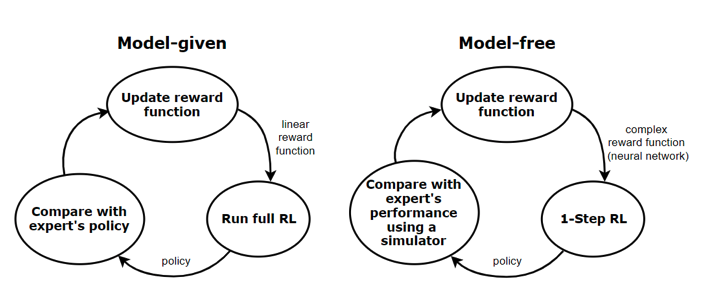
\includegraphics[width=\linewidth]{fig/IRL.png}}
        \end{figure}
\end{frame}


\begin{frame}{Dilemma of data-driven scientific computing}
	In the data-driven scientific computing, \textcolor{red}{\textbf{dynamics structure}} can cause \textcolor{red}{\textbf{distribution mismatch}} between the training and testing data.
	\begin{figure}[H]
          \centering
          \centerline{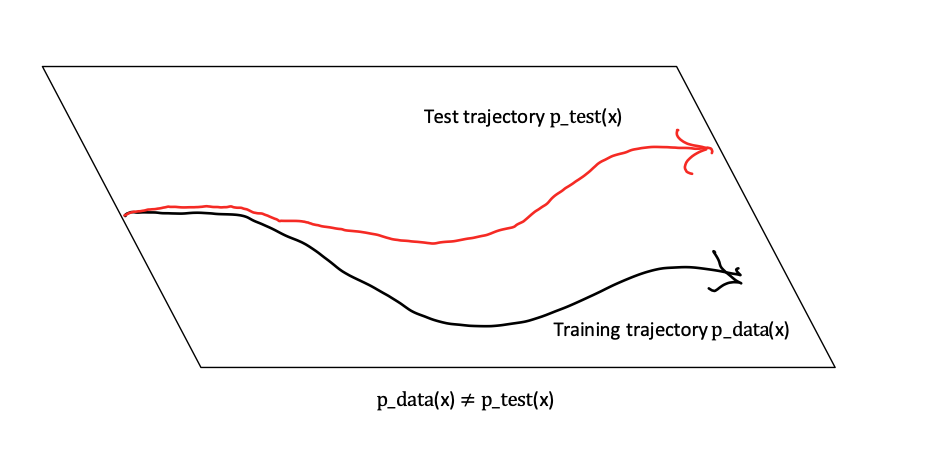
\includegraphics[width=\linewidth]{fig/dilemma.png}}
        \end{figure}
\end{frame}


\begin{frame}{Algorithm to mitigate the distribution mismatch}
	Modified the training dataset to mitigate the distribution shift.
	\begin{figure}[H]
          \centering
          \centerline{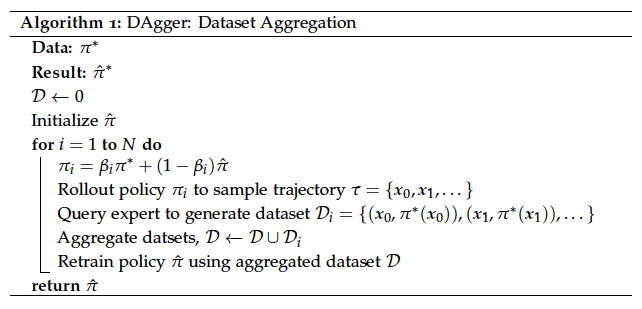
\includegraphics[width=\linewidth]{fig/DAgger.png}}
        \end{figure}
\end{frame}


\begin{frame}{Algorithm to mitigate the distribution mismatch}
	\begin{figure}[H]
          \centering
          \centerline{\includegraphics[width=\linewidth]{fig/DAggerpic.png}}
        \end{figure}
\end{frame}


\begin{frame}{Algorithm to mitigate the distribution mismatch}
	Design network model based on physical principles to enhance its stability.
	\begin{figure}[H]
          \centering
          \centerline{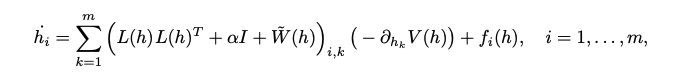
\includegraphics[width=\linewidth]{fig/onsager1.png}}
        \end{figure}
        \begin{figure}[H]
          \centering
          \centerline{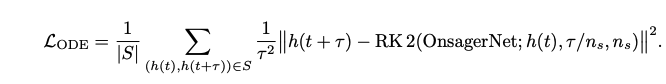
\includegraphics[width=\linewidth]{fig/onsager2.png}}
        \end{figure}
        \footnotetext{Yu, Haijun, et al. "OnsagerNet: Learning stable and interpretable dynamics using a generalized Onsager principle." Physical Review Fluids 6.11 (2021): 114402.
}
\end{frame}


\begin{frame}{An intuition}	
	\bequn
		\begin{aligned}
			\p_t \mfx & = \mcL(\mfx, \mfu, t), \quad \mfx \in \mcX, \mfu \in \mcU, \mcL: \mcX \times \mcU \times \mbR_+ \rightarrow T\mcX,			\\
			\mfu & = \phi(\mfx, t), \quad \phi: \mcX \times \mbR_+\rightarrow \mfu.
		\end{aligned}
	\eequn
	Ordinary least square $\norml \mfu - \phi(\mfx, t) \normr^2$ cannot distinguish the following case. Add regularization for this as $R(\wht \mfx)$.
	\begin{figure}[H]
          \centering
          \centerline{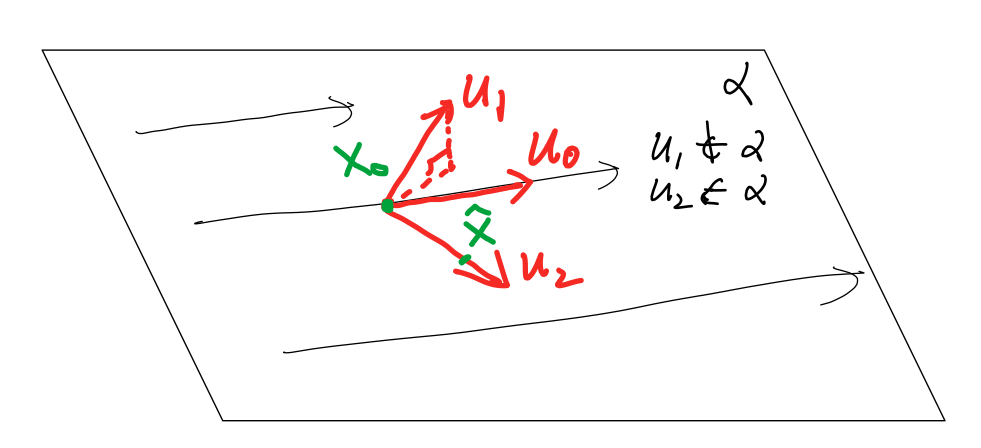
\includegraphics[width=\linewidth]{fig/mfd.png}}
        \end{figure}
\end{frame}


\begin{frame}{Algorithms and numerical experiments}
	Linear control:
	\begin{equation}
    \begin{aligned}
        \dot{x}_t & = v_t, \\
        \dot{v}_t & = -\alpha(t) v_t + u_t,	\\
        	x_0 & = 1, v_0 = 0,		\\
	x_1 & = 0,			\\
	\alpha(t) & = \sin 10 t.
    \end{aligned}
\end{equation}
And we use a \textbf{neural network} with $2$ hidden layer to parameterize the mapping from $(x_k, v_k, t_k)$ to $u_k$. Hence the neurons in each layer is given by $3, n, n, 1$ where $n$ can be varied in the experiments.
\end{frame}


\begin{frame}{Algorithms and numerical experiments}
	Inner-Outer loop structure of this linear control:
	\begin{equation}
		\begin{aligned}
			\begin{pmatrix} x_{k+1} \\ v_{k+1}
			\end{pmatrix} & \ = \begin{pmatrix} 1 & dt \\ 0 & 1-\alpha_k dt
			\end{pmatrix}\begin{pmatrix} x_{k} \\ v_{k}
			\end{pmatrix} + \begin{pmatrix} 0 \\ 1
			\end{pmatrix}u_k,		\\
			u_k & \ = \phi_{NN}(x_k, v_k, t_k).
		\end{aligned}
	\end{equation}
	And ordinary least square (behavior cloning) simply solve the model by minimizing the following function:
	$$l(\phi_{NN}(x_k, v_k, t_k), u_k) = \norml \phi_{NN}(x_k, v_k, t_k) - u_k \normr_2^2.$$
\end{frame}


\begin{frame}{Bench mark: Ordinary least square}
	Averaged error is given by $0.192341$.
	\begin{figure}[H]
          \centering
          \centerline{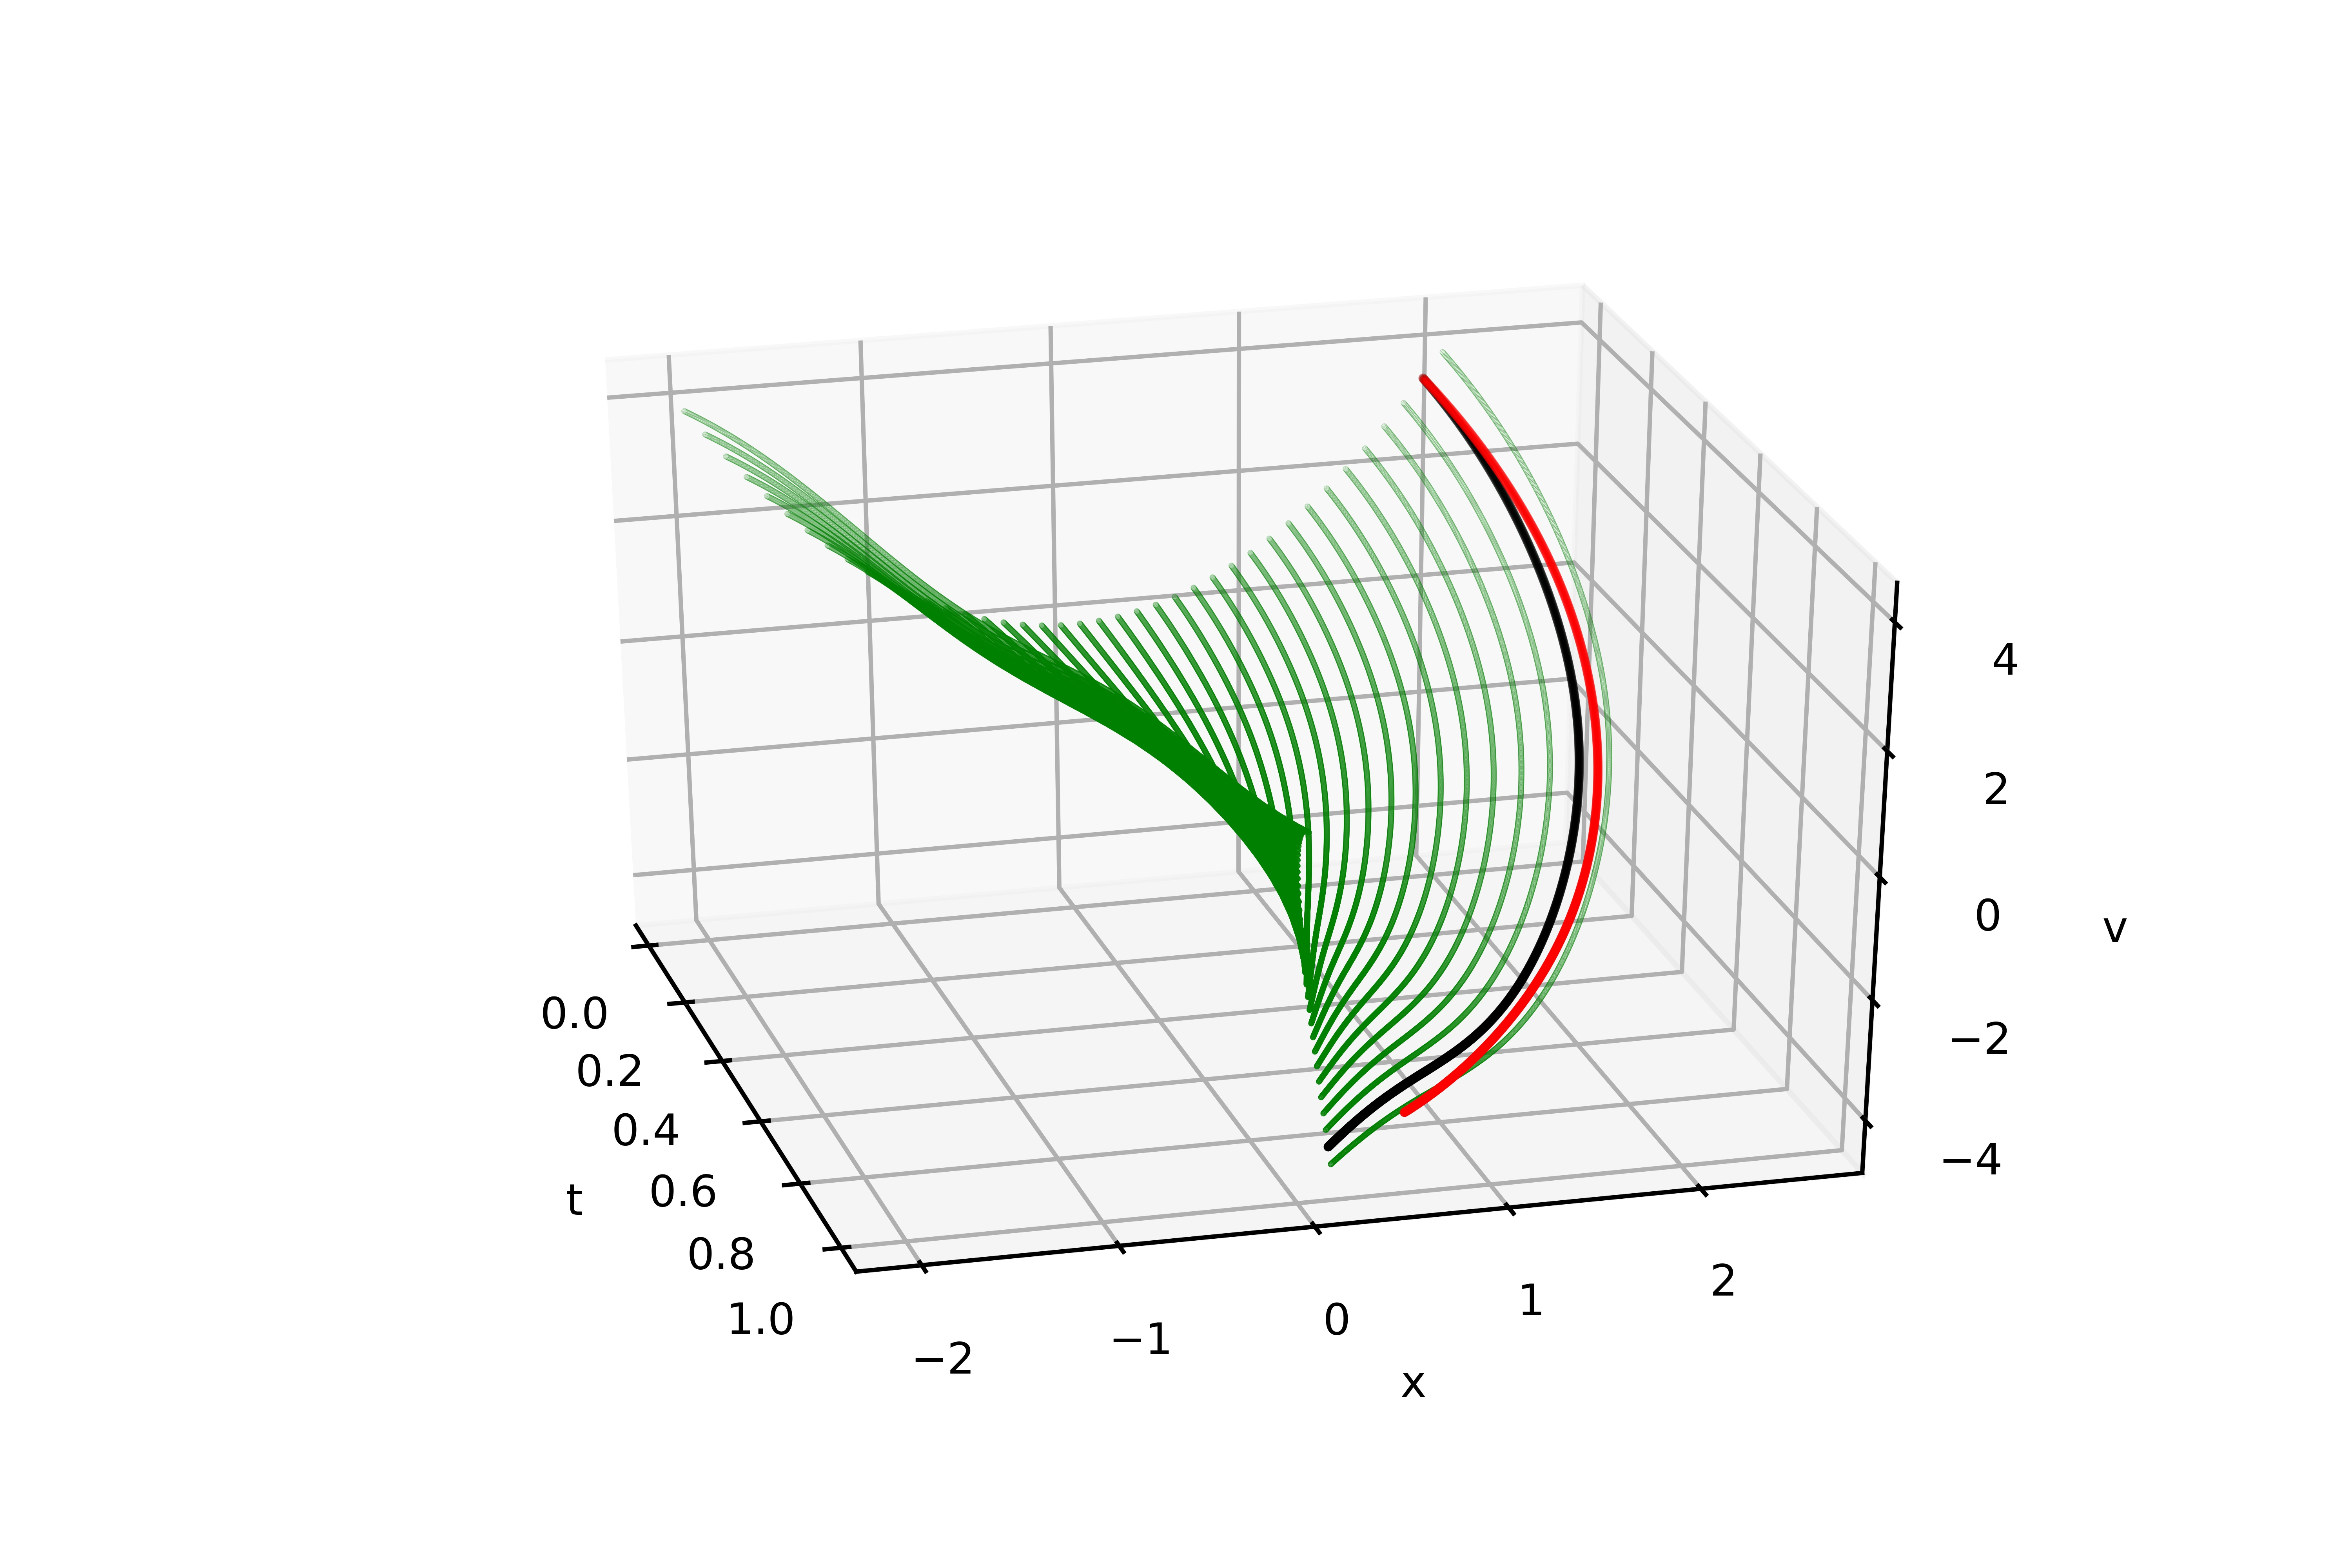
\includegraphics[width=0.7\linewidth]{fig/control1-1.jpg}}
          \caption{Sampled training trajectory of an estimator with underlying net of 		10 hidden neurons.}
	\end{figure}
\end{frame}


\begin{frame}{Manifold regularization}
	Several choices of empirical manifold:
	\begin{itemize}
		\item Formed by the sample trajectories in the training data, i.e.
	\bequn
		\mcM_t := \lbb (x(t), v(t), t)  \quad t \in [0, 1]  \rbb,
	\eequn
		\item The other empirical manifold related to the data-driven surrogate model and can be defined as following set:
\bequn
	\wht \mcM_t := \lbb (x, v, t) \Big| \norml \phi_{NN}(x_k, v_k, t_k) - u_k \normr_2 < \epsilon \rbb.
\eequn
	
\end{itemize}
\end{frame}


\begin{frame}{$ \mcM_t $}
\bequn
		\min_{\theta} \mbE \norml \mfu - \phi_{\theta}(\mfx, t) \normr^2 + \lambda \norml D(E(\wht \mfx)) - \wht \mfx \normr^2
	\eequn
	Averaged error is given by $0.173001$.
	\begin{figure}[H]
          \centering
          \centerline{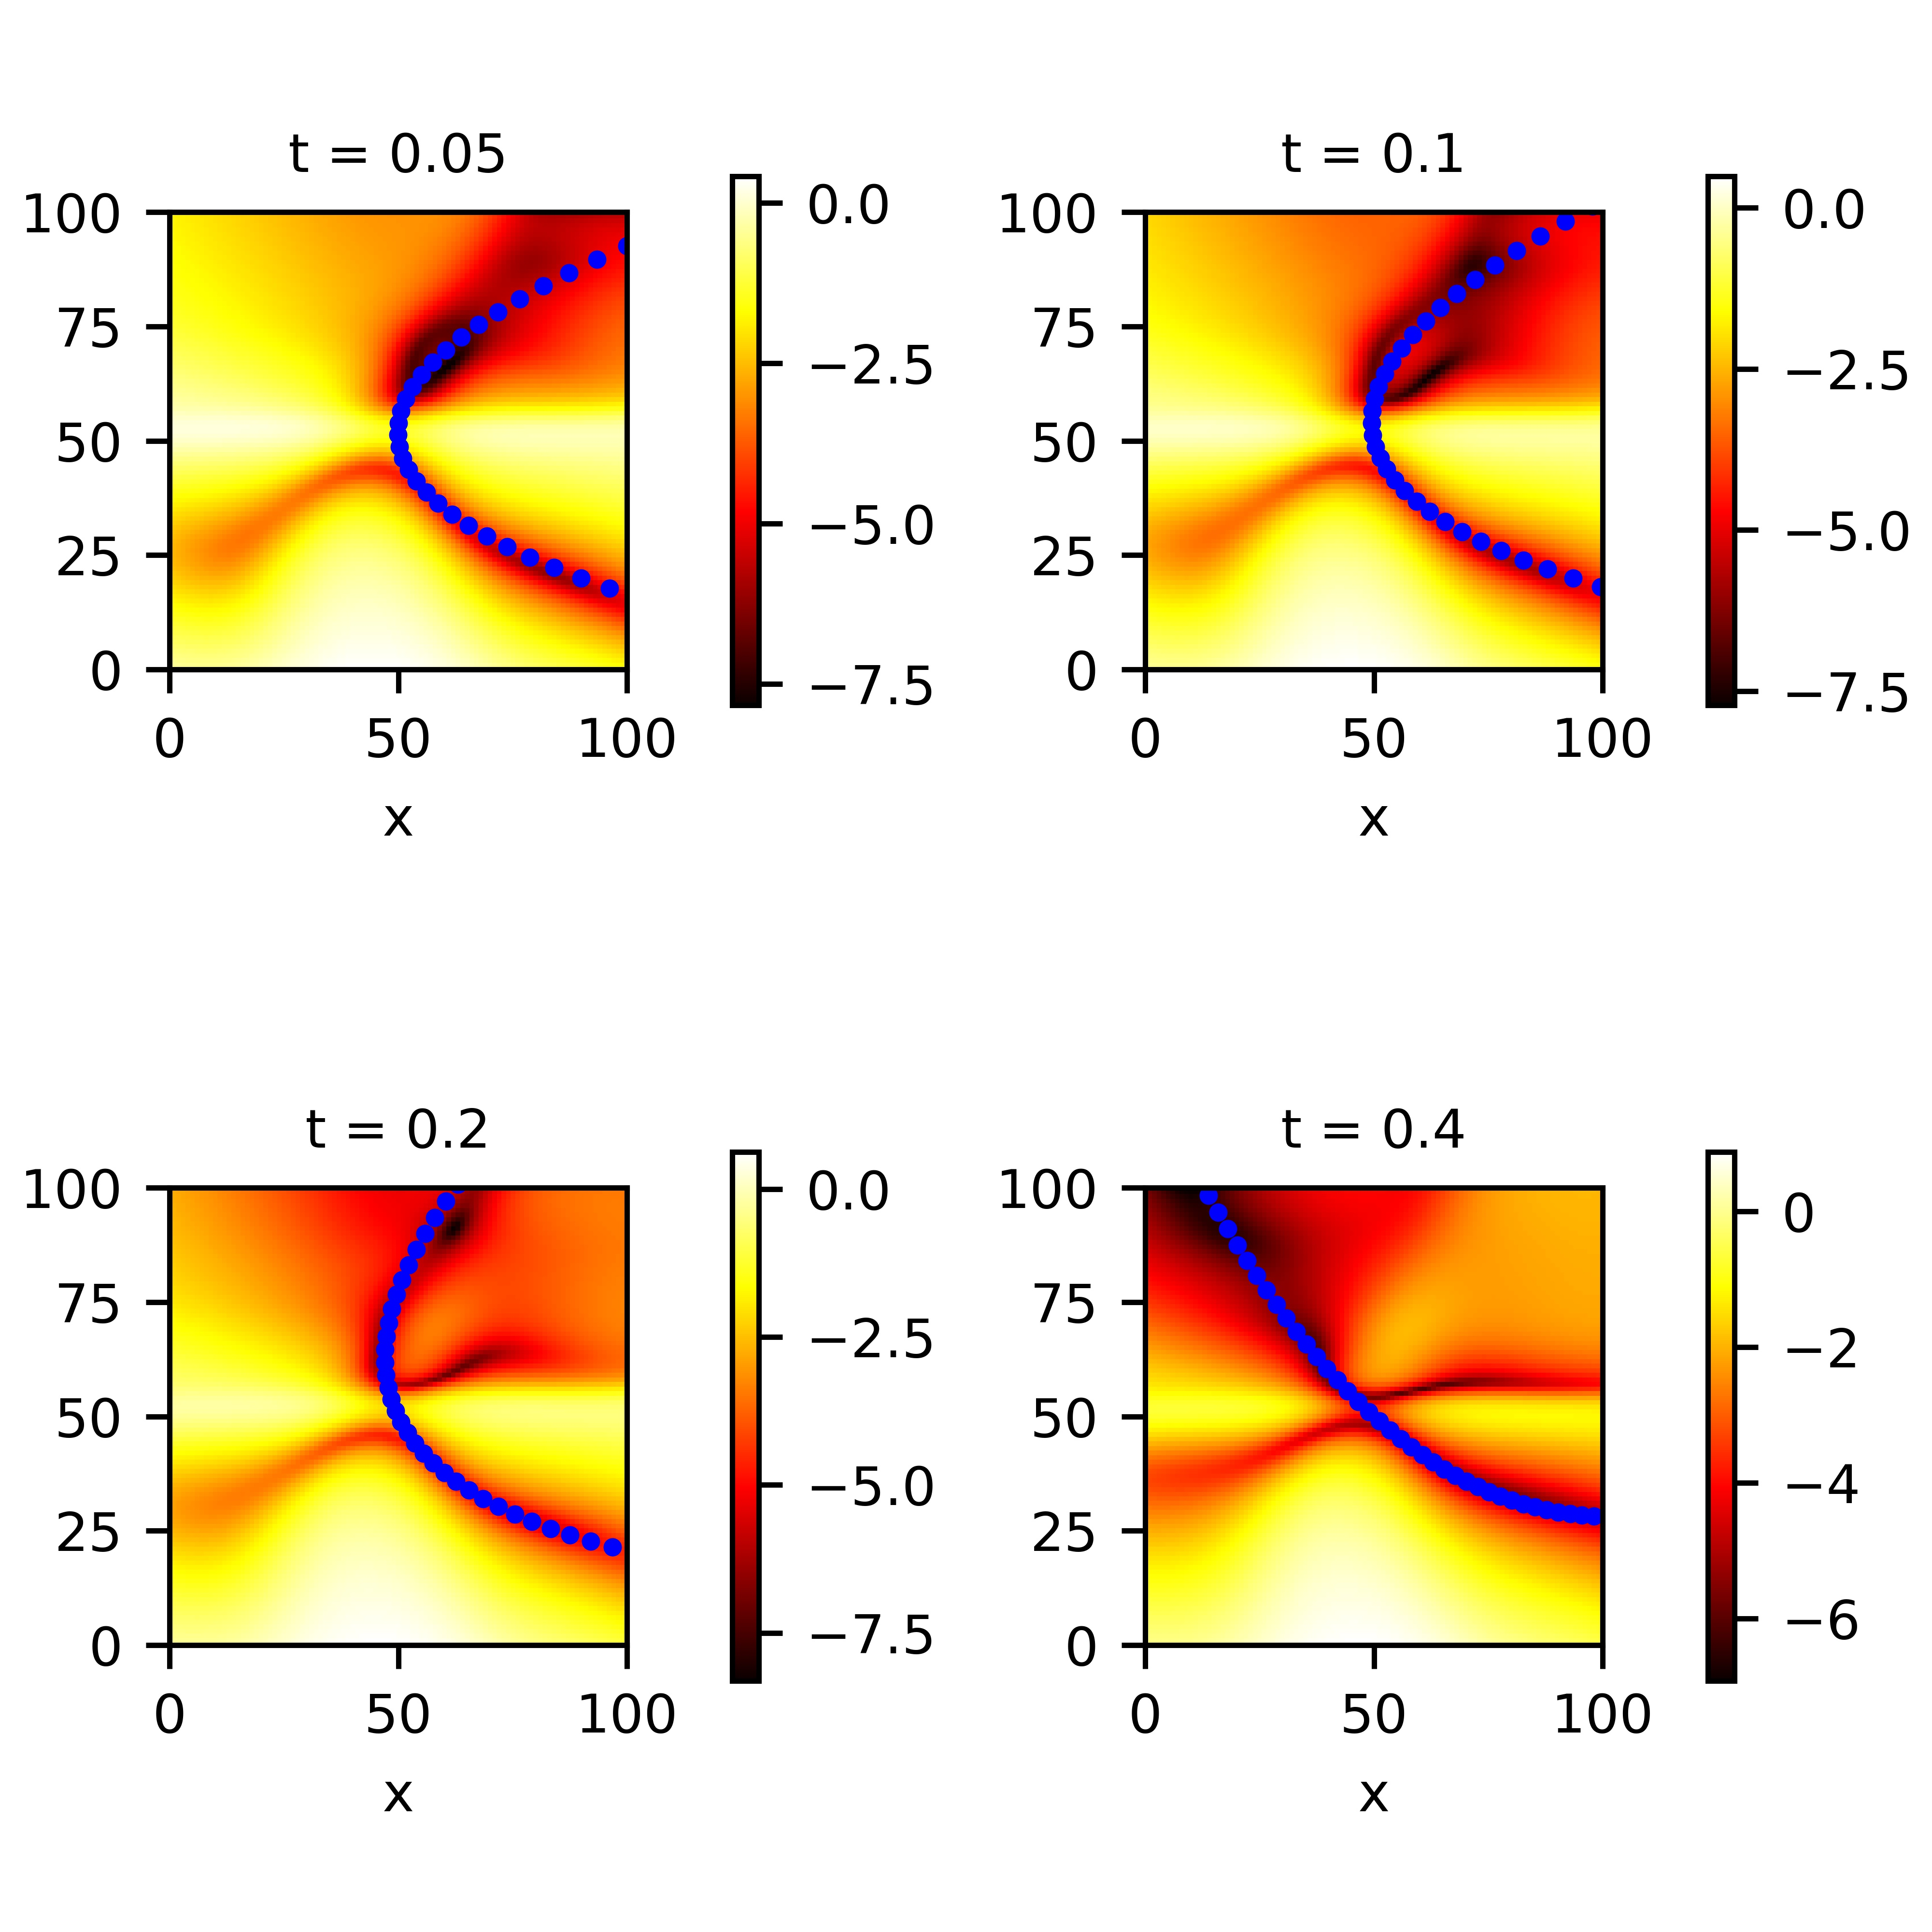
\includegraphics[width=0.65\linewidth]{fig/control6.jpg}}
          \label{l2-mfd}
\end{figure}
\end{frame}


\begin{frame}{$\wht \mcM_t $}
	\bequn
		\min_{\theta} \mbE \norml \mfu - \phi_{\theta}(\mfx, t) \normr^2 + \lambda \norml \wht \mfu - \phi_{\theta}(\wht \mfx, t) \normr^2
	\eequn
	Averaged error is given by $0.160128$.
	\begin{figure}[H]
          \centering
          \centerline{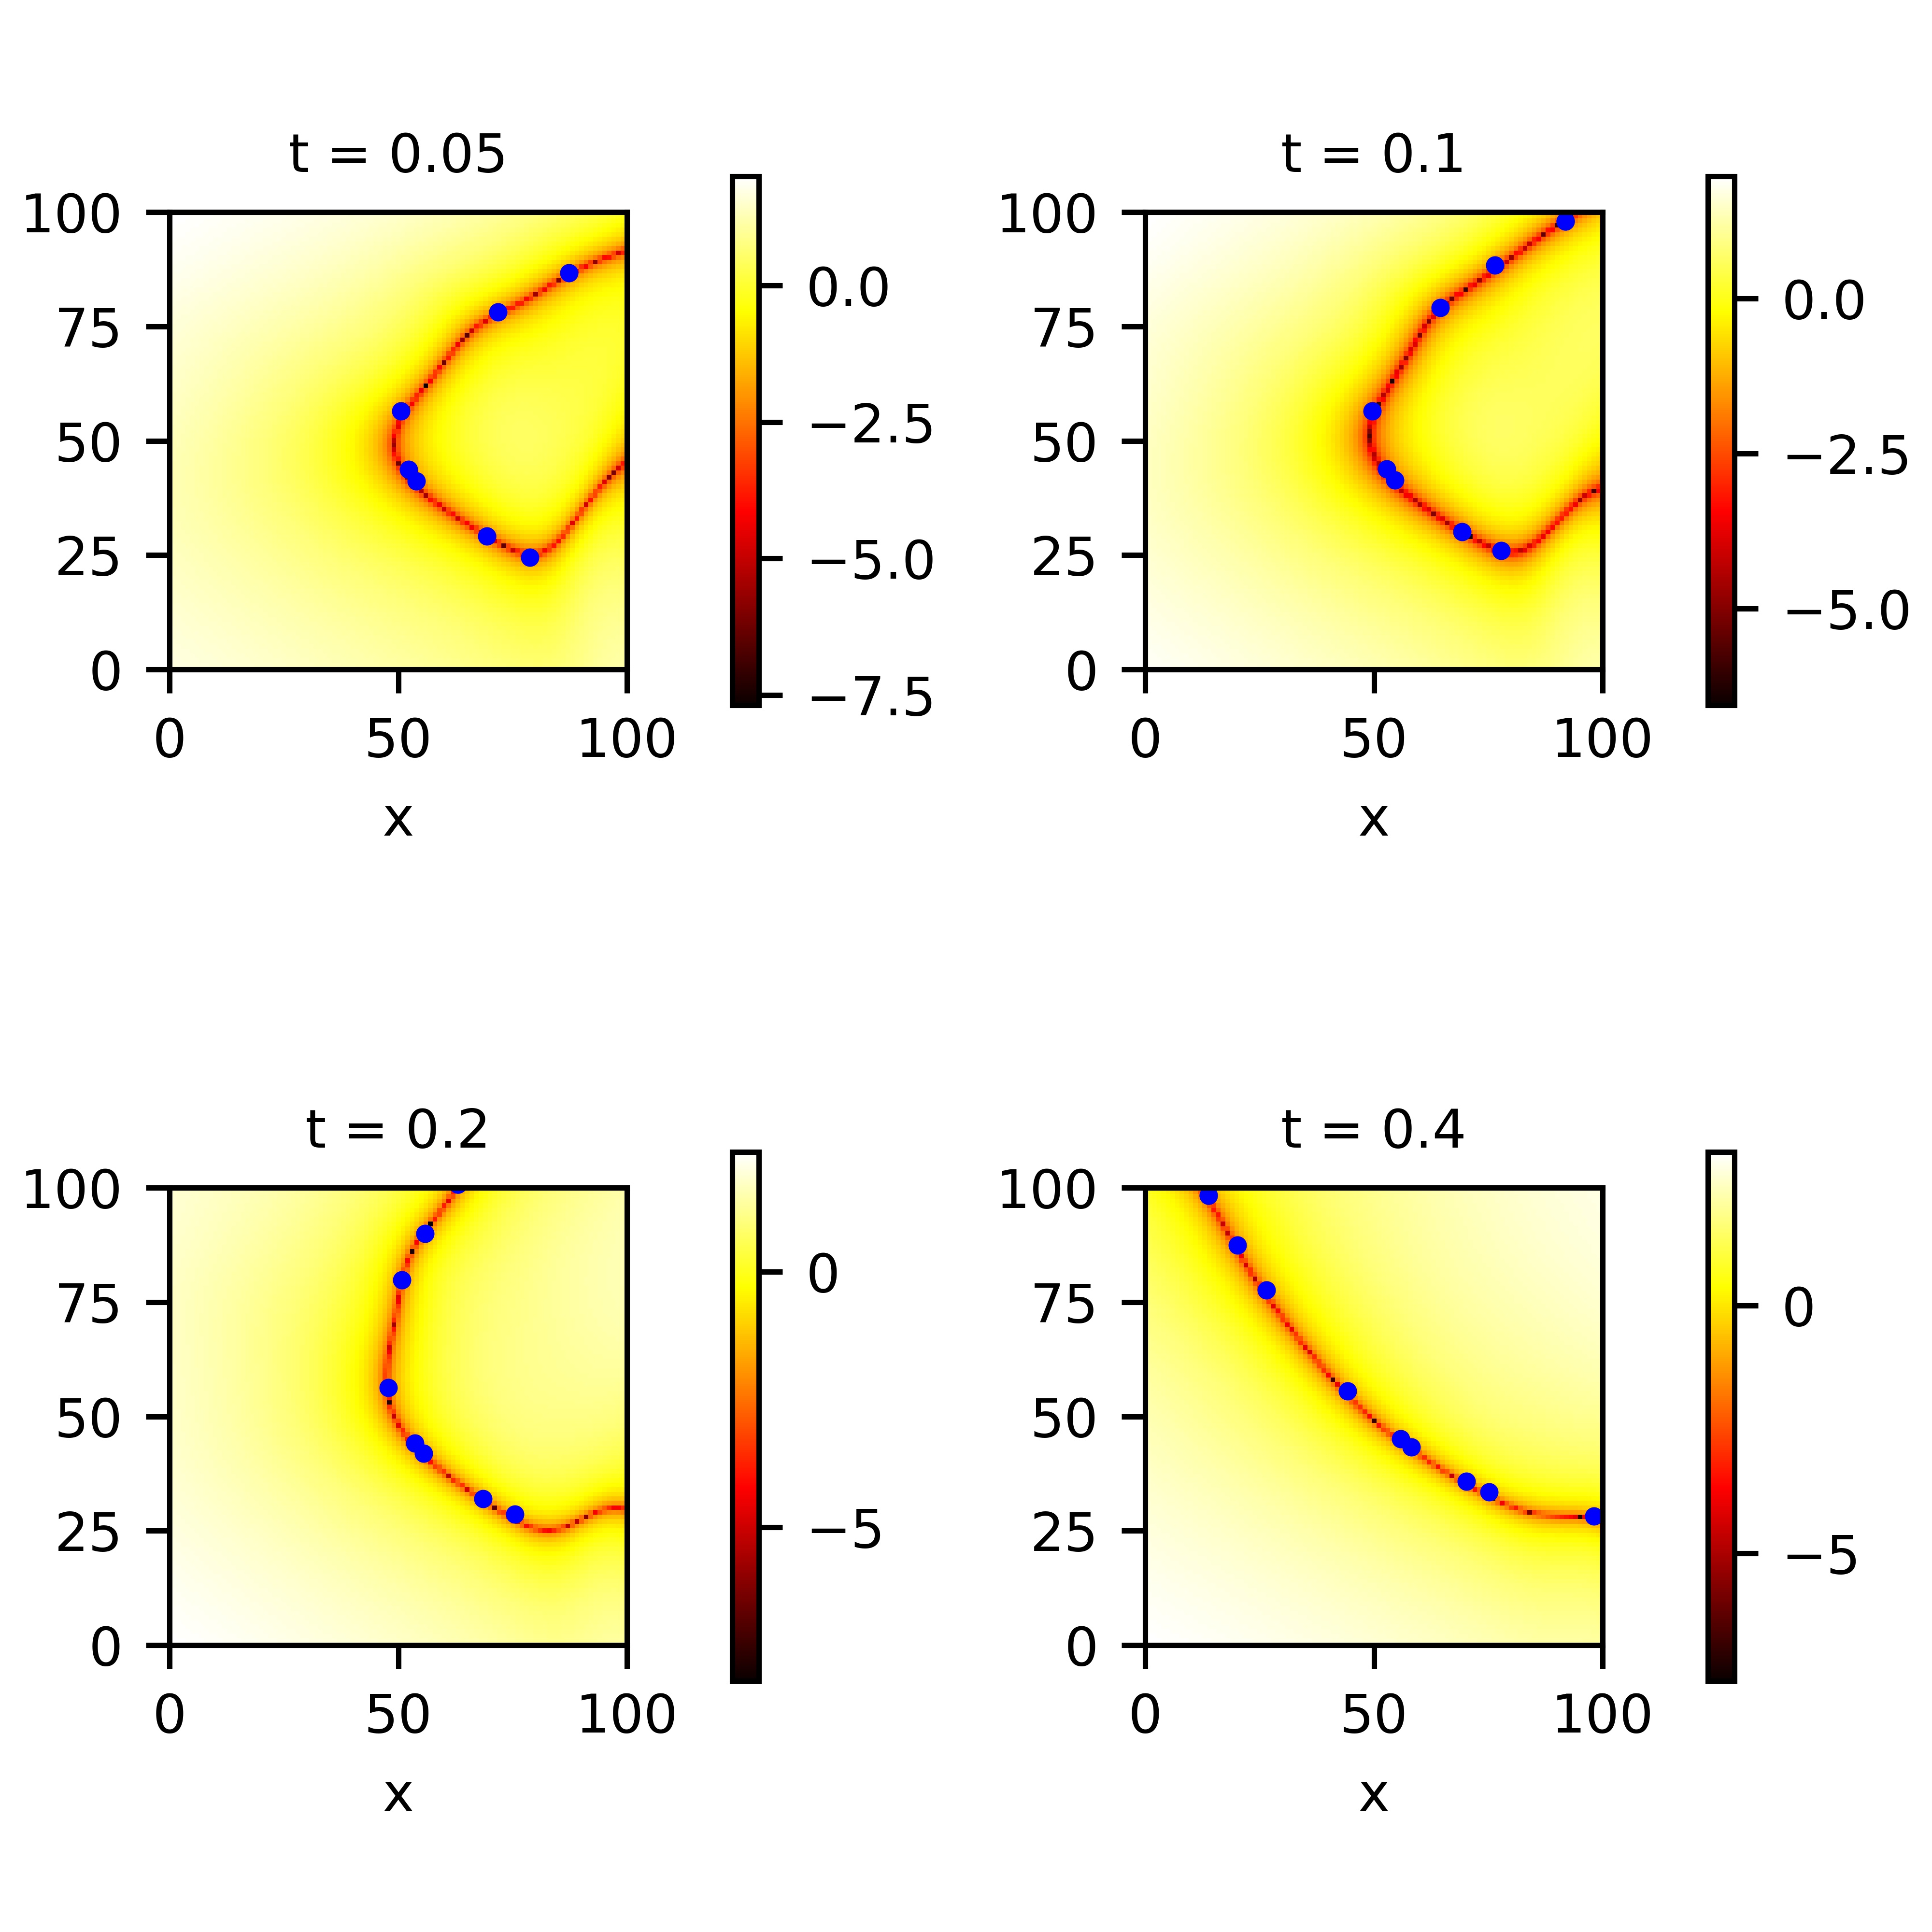
\includegraphics[width=0.65\linewidth]{fig/control4.jpg}}
          \label{l2-mfd}
	\end{figure}
\end{frame}


\begin{frame}{Future work: Algorithm}
In the algorithmic perspective
	\begin{itemize}
		\item 1. Complete the work on encoder-decoder regularized method to mitigate the distribution mismatch in scientific computing.
		\item 2. Scientific computing + Manifold learning/self-supervised learning.
	\end{itemize}

\end{frame}


\begin{frame}{Future work: Application}
	In terms of application, we will further investigate the following thing:
	\begin{itemize}
		\item 1. Try to implant the best performed algorithm to the problems in fluid mechanics such as turbulence transition and flow separation.
		\item 2. Consider interesting problems in physics such as black holes dynamics, space-time classification in general relativity.
	\end{itemize}

\end{frame}


\begin{frame}{Future work: Theory}
Theoretically, we will consider
	\begin{itemize}
		\item 1. Prove the effectiveness of the algorithm like Dagger and manifold learning method.
		\item 2. Consider algorithms belong to inverse reinforcement learning in our model-based setting.
	\end{itemize}

\end{frame}







\end{document}